\documentclass[a4paper]{report}

% Import packages
\usepackage{amsmath, amsfonts, amsthm}  % AMS math libraries
\usepackage{amssymb}       % Large extended set of symbols: http://home.online.no/~pjacklam/latex/textcomp.pdf
\usepackage{multirow}      % Row spanning in tables.
\usepackage{graphicx}      % Extended graphics library
%\usepackage{textcomp}      % Extended set of symbols: http://home.online.no/~pjacklam/latex/textcomp.pdf
%\usepackage{varioref}      % Use \vref instead of \ref
%\usepackage{wrapfig}
%\usepackage{subfigure}
%\usepackage{url}
\usepackage[pdftex,
	pdfauthor={Jan Magne Tjensvold},
	pdftitle={Generic Distributed Exact Cover Solver},
	pdfkeywords={Distributed; Computing; Distributed computing; Exact Cover; Dancing Links; DLX},
	pdfsubject={Distributed computing},
	pdflang={en},
	bookmarks,
	bookmarksnumbered,
]{hyperref}  % Sets pdfTeX to include bookmarks in the output file (Should always be the last package included)
\usepackage{algorithm}     % Pseudocode float environment
\usepackage{algorithmic}   % Pseudocode
\usepackage[noend, nobraces]{javadistalgo}  % Java style pseudocode

\graphicspath{{./}{images/}}

% Limit the depth of the table of contents
%\setcounter{tocdepth}{1}

% Custom commands

%\renewcommand{\bmod}{\mbox{ mod }}

%\makeatletter
%\def\imod#1{\allowbreak\mkern10mu({\operator@font mod}\,\,#1)}
%\makeatother

%\DeclareMathOperator{\lcm}{lcm}

% Document info
\title{Generic Distributed Exact Cover Solver}
\author{Jan Magne Tjensvold}
\date{\today}



% Here the actual document begins.
\begin{document}

\maketitle  % Report titlepage

% Include external file
%
\begin{abstract}
This report details the implementation of a distributed computing system which can be used to solve exact cover problems.
This work is based on Donald E. Knuth's recursive Dancing Links algorithm which is designed to efficiently solve exact cover problems.
A variation of this algorithm is developed which enables the problems to be distributed to a global network of computers using the BOINC framework.
The parallel nature of this distributed computing platform allows more complex problems to be solved.
Exact cover problems includes, but is not limited to, $n$-queens, Latin Square puzzles, Sudoku, polyomino tiling, set packing and set partitioning.
The details of the modified Dancing Links algorithm and the implementation is explained in detail.
A Petri net model is developed to examine the flow of data in the distributed system by running a number of simulations.
\end{abstract}

\cleardoublepage
\chapter*{Acknowledgements\markboth{Acknowledgements}{Acknowledgements}}
I wish to thank Hein Meling for his detailed and insightful comments on the report and his helpful ideas on the design and implementation of the software.
  % Abstract

% Table of contents, tables and figures
\tableofcontents
%\listoftables
%\listoffigures

% Include external files

\chapter{Introduction}

This report details the design and implementation of a distributed computing system to solve exact cover problems.
Donald Knuth's Dancing Links (DLX) algorithm \cite{knuth00dancing} is used to solve the exact cover problem.
Exact cover is a general type of problem which can be applied to a wide range of problems.
It can be used to solve problems like $n$-queens, polyomino tiling, Latin square puzzles, Sudoku, set packing and set partitioning.
For more detailed information about how exact cover can be applied to $n$-queens, polyomino tiling, Latin square and Sudoku, see Section \ref{transforms}.

Distributed computing with this algorithm is accomplished by exploiting the recursive nature of DLX to split the problem into smaller pieces.
The Generic Distributed Exact Cover Solver (DECS) then takes advantage of a distributed computing middleware called BOINC \cite{boinc} to handle the work distribution and result collection process.
The report explains in detail how the DLX algorithm works and some concrete types of problems it can be applied to.
It also explains how DLX is used together with BOINC to construct a complete distributed computing system.



\section{Queens}
\label{intro_queens}

The 8-queens problem asks how eight queens can be placed on an $8 \times 8$ chess board without leaving any of the pieces in a position to attack each other.
In chess a queen can attack horizontally, vertically and diagonally on the board.
Figure \ref{fig:8queens-invalid} might appear to be a valid solution at first sight, but more careful study shows that the queens at B1 and H7 are attacking each other, thus rendering this configuration invalid.
Figure \ref{fig:8queens} shows a valid solution to the eight queens problem.
Depending on the symmetries in the solution up to seven other solutions can easily be found by rotating the board 90, 180 and 270 degrees.
By turning the board upside down and applying the same rotations the other four solutions can be found.
The 8-queens problem has a total of 92 configuration where none of the queens attack each other.

$n$-queens is the generalized form of the 8-queens problem where $n$ queens are placed on an $n \times n$ board.
A number of different algorithms exist to find all the solutions to a given $n$-queens problem.
This report will show the details of how the DLX algorithm is able to solve the $n$-queens problem.

\begin{figure}[hptb]
	\centering 
	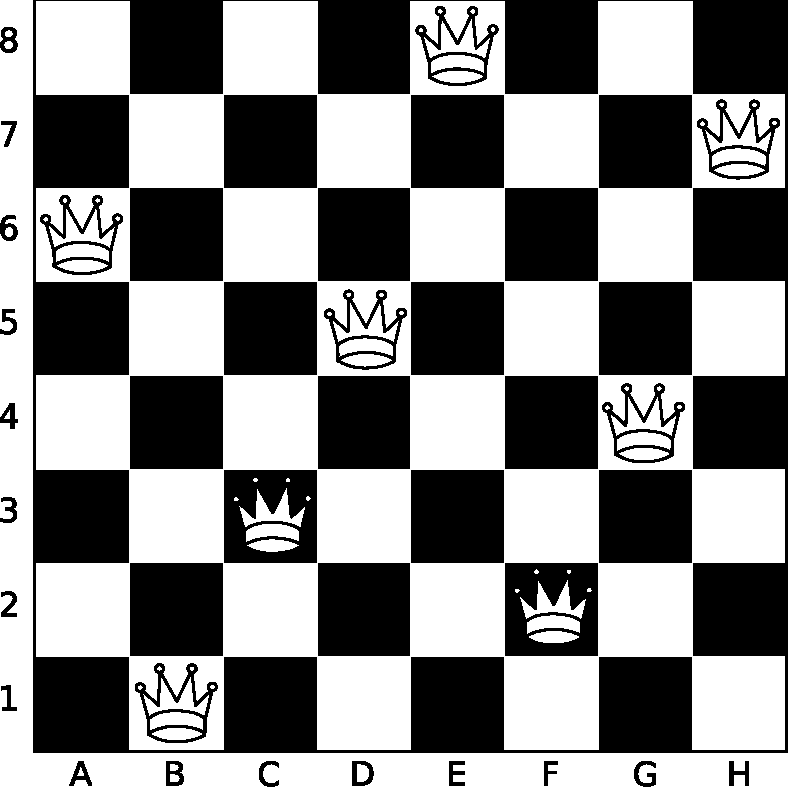
\includegraphics[width=0.65\textwidth]{queens-invalid.pdf}
	\caption{Board configuration where the queens at B1 and H7 attack each other}
	\label{fig:8queens-invalid}
\end{figure}

\begin{figure}[hptb]
	\centering 
	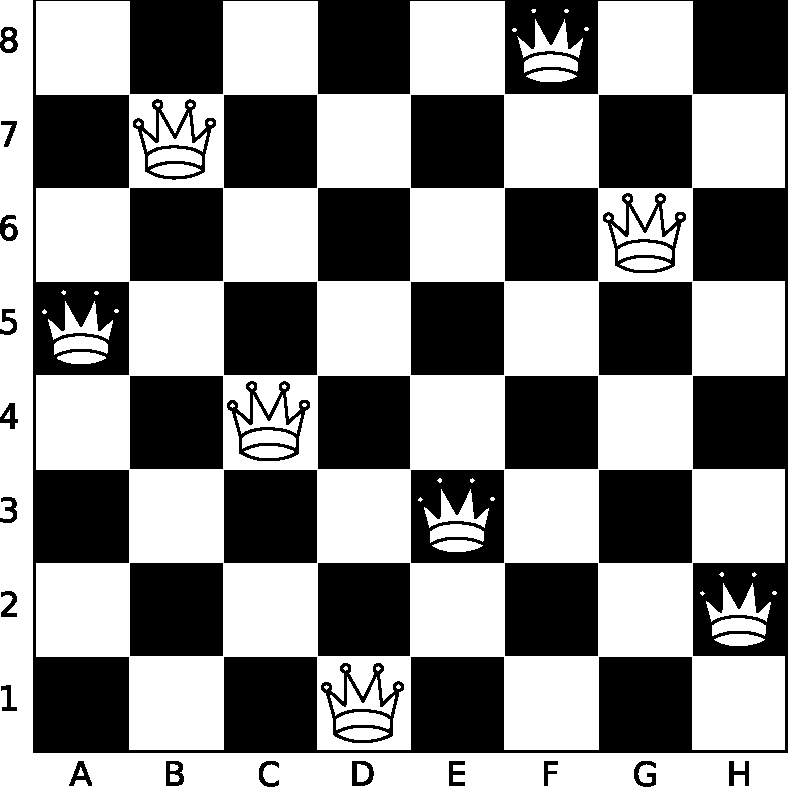
\includegraphics[width=0.65\textwidth]{queens-basic.pdf}
	\caption{One possible solution to the 8-queens problem}
	\label{fig:8queens}
\end{figure}



\section{Related work}

There are numerous implementations of the Dancing Links algorithm available with and without source code.
In addition to Knuth's own implementation in CWEB \cite{cweb} a quick search found source code for Java, Python, C, C++, Ruby, Lisp, MATLAB and Mathematica.
Some of the implementations were generic while others aimed for a specific application (mostly Sudoku).
Common for all these implementations is that none of them were designed for parallel processing.

Alfred Wassermann developed a parallel version of Knuth's algorithm in \cite{wassermann99covering} by using PVM \cite{pvm} to solve a problem presented in Knuth's original paper.
However, he only published the solutions to the problem and not the actual implementation.
The only available open source parallel version is written by Owen O'Malley for the Apache Hadoop project \cite{hadoop} in May 2007.
O'Malley's implementation uses the MapReduce framework \cite{map-reduce} provided by Hadoop to do the computations in parallel.
The details of this implementation and how it divides the problem into smaller pieces has to the author's knowledge not been published.



\section{Report organization}

This report is organized into several chapters.
Chapter \ref{dancing_links} describes the Dancing Links algorithm.
Chapter \ref{implementation} discusses different aspects of the implementation.
Chapter \ref{testing} describes the test results with the system and Chapter \ref{conclusion} concludes this report.


\chapter{Dancing Links}
\label{dancing_links}

% Description of Donald Knuth's Dancing Links (DLX) algorithm.


\section{Background}

% Other implementations of Dancing Links.
% Adobe Open Source: http://opensource.adobe.com/classadobe_1_1dancing__links.html
% - C++, general (not application specific), generic with secondary columns, has callback functionality passing a void function pointer, uses templates.
% - Mathematica Add-On, general, not generic, 

\section{Exact cover}


% Applications:
% Polyomino tiling
% Latin squares - Special types of latin squares can be used as error correcting codes for power line communication (sending radio signals over electric power lines) \cite{Colbourn04}
% Sudoku (special case of Latin squares)
% N-Queens
% set packing
% set partitioning

\cite{Colbourn04}
%
\chapter{Distributed computing}
\label{distributed_computing}

% Description of the distributed computing concept and what 3rd party software can be used to implement this concept.

%A Danish bachelor project from the spring of 2007 [http://code.google.com/p/queens/] tried to solve the $N$ queens problem for $N=26$ on the MiG [http://mig-1.imada.sdu.dk] Grid computing platform.


\section{History}


\section{Applications}


\section{BOINC}

Components of a BOINC server
\begin{itemize}
	\item Feeder
	\item Transitioner
	\item File deleter
	\item Application
	\item Work generator
	\item Validator
	\item Assimilator
\end{itemize}
%
\chapter{Implementation details}
\label{implementation}

% Here we describe some of the important implementation details.



\section{Transforms}


\subsection{N-Queens}

% [Begin Wikipedia quote] Consider a matrix with one column for each of the n ranks of the board, one column for each of the n files, and one column for each of the 4n-6 nontrivial diagonals of the board. The matrix has n^2 rows: one for each possible queen placement, and each row has a 1 in the  columns corresponding to that square's rank, file, and diagonals and a 0 in  all the other columns. Then the n queens problem is equivalent to choosing a subset of the rows of this  matrix such that every column has a 1 in precisely one of the chosen rows;  this is an exact cover problem. [end Wikipedia quote]

% Actually, the Wikipedia entry contains an error in the argumentation. On  an n by n board, we will place at most n queens. They will avoid each other by being in separate rows and columns.  But we have a total of 2n-3 parallel diagonals which have to be guarded by the n queens. Which means  that all diagonals will not be occupied. The exact cover procedure will not  find any solutions. So, in order to turn the problem into a correct exact  cover problem, we will add 4n-6 lines with a 1 only in each of the columns corresponding to the  diagonals. This will allow the algorithm to complete its search for a  complete cover by adding these rows, which we can then delete afterwards  (these will be the only rows with only a single column entry). 
% -- http://www.imtek.de/simulation//mathematica/IMSweb/imsTOC/Game%20Theory/ExactCoverDocu.html


\subsection{Polyominoes}


\subsection{Latin square}

% Application of Exact Cover to Solving the Latin Square Puzzle
% -- http://www.imtek.de/simulation//mathematica/IMSweb/imsTOC/Game%20Theory/ExactCoverDocu.html


\section{File format}

In order to store and transfer the DLX problem matrix efficiently a file format was defined for this specific purpose.

The file the DLX problem matrix is stored in had to be given a clearly defined format. 

%Challenges:
%- Byte ordering
%- Format version
%- Storage of the boolean matrix (for efficient operation we first need to find out how the circular quad linked list of objects are most efficiently built. From top-left to bottom-right.

%How to handle different byte ordering in the file format?
%Make the file format x86 centric by requiring all values to be stored as little-endian.
%Little end first, or increasing significance 
%\cite{IEN137}

\begin{table}[htbp]
	\centering
	\begin{tabular}{|r|r|l|p{2.7in}|}
		\hline
		\bf Offset & \bf Length & \bf Field & \bf Description \\ \hline
		0  & 4 & file\_id & File type ID: ``DECS'' \\ \hline
		4  & 1 & version & File format version. \\ \hline
		5  & 1 & & Reserved. \\ \hline
		6  & 1 & col\_bits & Number of bits used to represent column numbers + 1. \\ \hline
		7  & 1 & row\_bits & Number of bits used to represent row numbers + 1. \\ \hline
		8  & 4 & col\_count & Number of columns. \\ \hline
		12 & 4 & row\_count & Number of rows. \\ \hline
		16 & 4 & elem\_count & Number of non-zero values in the matrix. \\ \hline
		20 & 4 & names & Byte offset to the column and row name list. 0 if unavailable. \\ \hline
		24 & 4 & seccol & Byte offset to the secondary column list. 0 if unavailable. \\ \hline
		38 & 4 & elements & Byte offset to the matrix element entries. Should never be 0. \\ \hline
		32 & 4 & probid & Problem type ID. Each problem type has a unique ID so that the correct transform can be chosen and the problem specific information can be decoded. \\ \hline
		36 & 4 & probinfo & Byte offset to problem specific information. 0 if unavailable. \\ \hline
%		26 & 2 & Number & Job ID. Each problem type has a unique ID so that the correct transform is selected. \\ \hline
	\end{tabular}
	\caption{File header format}
	\label{tab:header}
\end{table}

The DLX algorithm itself does not use the column and row names or the problem type ID and the problem specific information.
This information can be used by the BOINC client to display graphical information during the computation.
For example it can use the problem type ID to identify the correct transform, and when the DLX algorithm finds a solution it can run the reverse transform and display the solution graphically.
BOINC has built-in support for OpenGL rendering and the solution can be displayed as part of a special BOINC screen saver.

By allowing the number of bits used to store the column and row numbers (col\_bits and row\_bits fields) to be an arbitrary integer we can achieve a reduction in file size without too much additional work.
Setting these parameters to something other than 8, 16 or 32 (or 64 on a 64-bit system) will incur an extra processing overhead when reading and writing the file as the program will have to apply some bit shifting operations to retrieve the values.
The trade off between processing overhead and file size can be beneficial in cases where the number of non-zero elements, rows and/or columns is large and where storage and bandwidth resources are scarce.
The number of bits for column and row numbers should always be large enough to accommodate the values of the maximum column and row numbers which is also specified in the file.
This means that the values of 


\begin{table}[htbp]
	\centering
	\begin{tabular}{|r|r|l|p{2.7in}|}
		\hline
		\bf Offset & \bf Length & \bf Type & \bf Description \\ \hline
		0  & 4 & Text   & File type ID: ``DECS'' \\ \hline
		4  & 1 & Number & Major file format version. Kernel like versioning. Even numbers are stable and odd numbers are experimental. \\ \hline
		5  & 1 & Number & Minor file format version. Files with same major version, but different minor are backwards compatible. \\ \hline
		6  & 2 &        & Reserved for future use. \\ \hline
		8  & 4 & Number & Number of columns. \\ \hline
		12 & 4 & Number & Number of rows. \\ \hline
		16 & 4 & Number & Number of non-zero values in the matrix. \\ \hline
		20 & 4 & Number & Byte offset to the column and row names. 0 if unavailable. \\ \hline
		24 & 4 & Number & Byte offset to the secondary column list. 0 if unavailable. \\ \hline
		28 & 4 & Number & Byte offset to the matrix element entries. Should never be 0. \\ \hline
		32 & 4 & Number & Problem type ID. Each problem type has a unique ID so that the correct transform can be chosen and the problem specific information can be decoded. \\ \hline
		36 & 4 & Number & Byte offset to problem specific information. 0 if unavailable. \\ \hline
%		26 & 2 & Number & Job ID. Each problem type has a unique ID so that the correct transform is selected. \\ \hline
	\end{tabular}
	\caption{File format for column and row names}
	\label{tab:header}
\end{table}



\subsection{Storing sparse boolean matrices}


\section{libdecs}


\subsection{Modes of operation}

% TODO: Fix this if we are able to return only the row numbers from the computing nodes (the DLX library).
DECS has two basic modes of operation regarding how it handles the return values of the system.
In the first mode, which is the most common, the system will store and forward all the solutions it finds back to the DECS server.
This provides the calling application with the full set of solutions so that it can run a detailed analysis on them or save them for later use.
For problems which generates a very large number of solutions or solutions which occupy large amounts of space this approach can cause a huge strain on the system.
The memory, storage and bandwidth capacities of the computing nodes and the DECS server could cause considerable delays.
In extreme cases it might even cause some or all of the solutions to never be returned.

A policy of not accepting overly large problem matrices could be implemented to prevent this problem.
This works well because the memory requirements of the DLX algorithm is proportional to the size of the problem matrix.
However, it does not do us much good because the problem will remain unsolved.

The second mode of operation will simply discard the solution matrices, but it keeps a count on the number of solutions
It will only keep a count

A possible extension to this would be to add other return values than number of solutions.
Each solution the DLX algorithm arrives at could be further analyzed so that other aspects of the solutions could be returned.



\section{BOINC}

\subsection{Architecture}


\section{libdlx}



%
\chapter{Test results}
\label{testing}

% Description of what tests has been performed.


\section{Simulation}

\cite{Tjensvold07-GPenSim}



\section{Performance}



%
\chapter{Conclusion}
\label{conclusion}

% Description of important/interesting implementation details.



\section{Future work}

\subsection*{Implement a compression scheme}

To ease the file format explanation and implementation no compression technique was implemented.
In cases where an exact cover problem has a very large number of solutions it would be an advantage to have some sort of compression.
A technique called bit packing described in \cite{gdip_bitpack, gpg_bitpack} provides a way to do some simple compression with a very low performance overhead.
By applying this technique we can exploit the otherwise unused bits.
The bit packing scheme can also be generalized to pack the data even more densely by doing sub-bit precision packing.
The trade off between processing overhead and file size can be beneficial in cases where the number of solutions is large and where storage and bandwidth resources are scarce.
It might also be worth looking into other compression schemes which are easy to implement.


\subsection*{Implement more transforms}

Currently only the $n$-queens transform has been implemented.
The other transforms explained in the report could be implemented as well making DECS more useful.


\subsection*{Improve the Petri net simulation model}

The Petri net model could be made more complete by incorporating other aspects of distributed computing as well.
Simulating client failure or malicious clients submitting incorrect data could be a possible extension.
That would require a certain piece of the problem to be sent to multiple clients for redundancy and verification.
It would also be a good idea to try to eliminate some of assumptions currently present in the simulation.
This would make the simulation results more accurate and true to the actual system.




%\subsection*{Implement a matrix hashing function}

%To 
% TODO Describe caching idea.
% Equivalence of matrixes with same solutions. Translations give same matrix, etc.



% How to organize the report:
% - Describe what problem or type of problem we are trying to solve and why.
% - Describe how we are going to solve it.
%   - The DLX algorithm.
%   - The Grid computing system for distributing the workload.
% - Describe some of the important implementation details.
% - Describe test results.



% BibTeX compiles the bibliography
\phantomsection
\addcontentsline{toc}{chapter}{\bibname}
\bibliographystyle{custom-r2}  % custom bibliography style
\bibliography{local}  % import local.bib

\end{document}